\section{Equipes de Fórmula SAE}

A Fórmula SAE é uma competição estudantil de âmbito mundial, organizada no Brasil
pela SAE Brasil e realizada anualmente \cite{sae_brasil_formula_sae}. As equipes
são compostas por alunos de uma mesma universidade, que ao longo do ano projetam,
constroem e testam um protótipo de veículo monoposto de competição. Na edição de
2025, a competição brasileira contou com 66 equipes inscritas, representando 64
instituições brasileiras de ensino superior de 11 estados e do Distrito Federal,
além de duas equipes do exterior \cite{sae_brasil_formula_sae_2025_inscritos}.

A competição é estruturada em provas estáticas e dinâmicas. As provas estáticas
avaliam o projeto de engenharia, o plano de negócios e o detalhamento de custos e
manufatura; as provas dinâmicas testam o desempenho do protótipo em situações como
aceleração, \emph{skidpad}, \emph{autocross} e \emph{endurance}. A prova de \emph{endurance} tem maior peso na
pontuação e exige que o veículo percorra aproximadamente 22 km sem falhas
\cite{fsaeonline_endurance_2026}.

Entre as equipes que participam da Fórmula SAE, a EESC-USP Formula SAE é o caso
estudado neste trabalho. Vinculada à Escola de Engenharia de São Carlos (EESC) da
Universidade de São Paulo (USP), a equipe reúne estudantes de vários cursos para
projetar, manufaturar e testar protótipos em competições nacionais e
internacionais \cite{eesc_usp_formula_sae_e22_2025}. Seu título mais recente foi
conquistado em 2025, quando venceu a categoria Combustão da 21ª Competição
Nacional de Fórmula SAE Brasil, garantindo vaga para a etapa mundial
\cite{eesc_usp_formula_sae_2025,sae_brasil_resultados_combustao_2025}.

\section{Aquisição de Dados no Veículo}

Em ambientes de competição automotiva, compreender o comportamento do veículo é
condição essencial para orientar ajustes de projeto, \emph{setup} e pilotagem. Sensores
distribuídos ao longo do protótipo fornecem informações que permitem validar
hipóteses de engenharia, monitorar sistemas críticos e comparar objetivamente
sessões de teste e desempenho entre pilotos
\cite{schultz2017_formula_sae_telemetry,ashford2020_formula_sae_data_analysis}.
Sem instrumentação adequada, a equipe depende principalmente do \emph{feedback} subjetivo
dos pilotos, que é útil, mas insuficiente para decisões de engenharia que precisam ser baseadas em dados confiáveis e
objetivos.

A aquisição de dados converte observações qualitativas em grandezas mensuráveis,
como pressão de freio, curso de suspensão, ângulo de esterço, aceleração lateral e
temperatura de óleo. Esses sinais ajudam a identificar onde o carro perde tempo,
avaliar se uma alteração teve o efeito esperado e registrar o comportamento do
protótipo ao longo da temporada. Trabalhos acadêmicos em Fórmula SAE mostram
soluções de baixo custo que combinam armazenamento local, comunicação sem fio e
visualização em tempo real
\cite{stoffman2004_low_cost_racing_daq,visconti2019_formula_sae_telemetry,zanetti2013_formula_sae_wireless,lauro2021_formula_sae_telemetria}.

No caso da EESC-USP, o sistema de aquisição de dados foi consolidado ao longo de
vários anos de desenvolvimento e testes, em continuidade a trabalhos anteriores de
eletrônica embarcada para Fórmula SAE. A arquitetura atual utiliza dois módulos
de aquisição com microcontroladores STM32, interligados por um barramento CAN a
1 Mbit/s, que também conecta outros módulos eletrônicos do veículo. Esse arranjo
parte da rede CAN estabelecida por Silva e de desenvolvimentos posteriores da
eletrônica da equipe documentados por Blatt
\cite{silva2009_rede_can_formula_sae,blatt2020_aquisicao_formula_sae}. Cada módulo lê
sensores analógicos e digitais instalados no carro e transmite os dados pela rede
CAN; os registros são armazenados em cartão SD embarcado e depois processados em
ferramentas de análise.

\section{Motivação}

Embora o sistema de aquisição da equipe seja robusto e consolidado, sua arquitetura
cabeada impõe restrições estruturais que limitam a capacidade de instrumentação
do veículo. O problema não está nos pontos de medição já consolidados, mas na
expansão da instrumentação para regiões em que o chicote passa a impor massa,
complexidade de montagem, interferência mecânica ou dificuldade de integração
com o fluxo de aquisição existente. Parte dessas limitações, envolvendo
componentes rotativos e superfícies aerodinâmicas do veículo, é ilustrada na
Figura~\ref{fig:can-cabeamento}. Essa tensão entre robustez de redes cabeadas e
flexibilidade de sensores sem fio também é discutida em estudos sobre redes
veiculares e intra-veiculares sem fio
\cite{blatt2020_aquisicao_formula_sae,tavares2008_wsn_automobiles,rahman2017_intravehicular_wsn,hashemi2014_intracar_multihop_wsn}.

\begin{figure}[htbp]
\centering
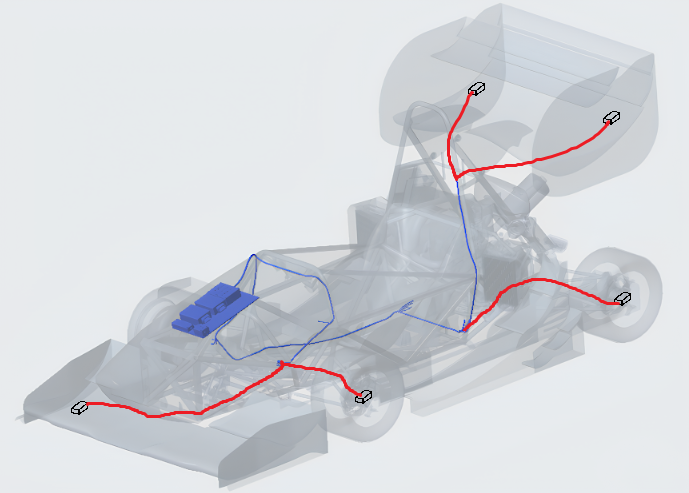
\includegraphics[width=0.85\textwidth]{images/can}
\caption{Dificuldades de roteamento e chicotes físicos para pontos de medição complexos no sistema cabeado atual. As linhas vermelhas indicam derivações de chicote dedicadas, as linhas azuis indicam trechos do chicote principal e os marcadores destacam pontos de instrumentação.}
\label{fig:can-cabeamento}
\end{figure}

Uma das situações mais restritivas ocorre nas regiões móveis próximas às rodas,
incluindo componentes rotativos e elementos ligados à transmissão, suspensão e
direção. Em componentes com rotação relativa, como o semieixo, a conexão com o
chicote elétrico do veículo é tecnicamente possível por meio de acopladores
rotativos, porém a complexidade de instalação, o custo e a fragilidade desses
componentes em ambiente de competição tornam a solução pouco atrativa. Isso
dificulta a leitura de sensores como temperatura de cubo ou torção do semieixo,
informações de alto valor para a dinâmica veicular. O semieixo transmite torque
entre o diferencial e a roda e acompanha a rotação do conjunto, tornando a
instrumentação com \emph{strain gauge} especialmente interessante para medir
deformações torsionais e inferir carregamentos aplicados durante a aceleração e
transientes de transmissão.

Além da limitação física, há também uma limitação temporal: a equipe trabalha hoje
com frequências fixas por identificador CAN, em geral na faixa de 200 Hz. Essa prática
funciona bem para a maioria dos canais, mas, no caso específico do semieixo, a equipe
pretende investigar se sinais associados à torção e a transientes de transmissão exigem
margem de aquisição maior. O valor de 1000 Hz usado nos ensaios deste trabalho não é
derivado de um modelo mecânico do semieixo; ele foi adotado como limite exploratório,
cinco vezes acima da frequência usual da equipe, para avaliar a margem prática da
camada WCAN. Pela relação de Nyquist
\cite{oppenheim1999_discrete_time_signal_processing}, a taxa de amostragem precisa ser
compatível com a maior frequência presente no sinal para evitar perda de informação,
mas a definição da banda mecânica útil ainda depende de ensaios específicos do
componente.

Limitações semelhantes aparecem em regiões onde o cabeamento pode interferir no
fenômeno a ser medido ou onde seu custo de instalação não se justifica pela
frequência de uso. A asa traseira é um exemplo relevante: por ser um componente
aerodinâmico, qualquer chicote exposto ao escoamento ou mal integrado à montagem
pode se tornar uma perturbação adicional ou uma restrição de instalação. Além
disso, testes de instrumentação na asa são pontuais e pouco frequentes, o que
torna menos justificável o investimento em um chicote dedicado, tanto em termos
de material quanto de mão de obra para montagem e desmontagem a cada sessão.

A mesma dificuldade de integração aparece quando a medição extrapola os limites
físicos do veículo. Sensores posicionados fora do carro, como um sensor de
passagem para detecção automática de voltas, ou equipamentos de medição
estacionários utilizados em testes controlados, não têm como se comunicar com o
sistema de aquisição embarcado por meios cabeados. Essa limitação dificulta a
integração de dados externos ao fluxo de aquisição, obrigando a equipe a
recorrer a registros manuais ou sistemas completamente separados, sem
sincronização temporal com os demais canais do carro.

Essas limitações motivam uma ponte CAN sem fio: um enlace dedicado à aquisição de
dados que reduza a dependência de cabeamento em pontos difíceis, mas preserve a
organização lógica por identificador CAN usada pelo sistema atual. A proposta não
busca substituir o barramento CAN físico do veículo, e sim estender o fluxo de
aquisição para cenários nos quais o cabeamento deixa de ser a alternativa mais
adequada.

\section{Objetivos e Contribuições}

O objetivo geral deste trabalho é desenvolver e avaliar, em bancada, uma ponte CAN
sem fio para aquisição de dados em Fórmula SAE. A proposta busca reduzir a
dependência de cabeamento em pontos de medição difíceis, usando o identificador CAN como referência lógica dos sinais e preservando compatibilidade conceitual com o
fluxo de aquisição já usado pela equipe.

Os objetivos específicos são:

\begin{itemize}
    \item caracterizar o problema e os requisitos de uma ponte CAN sem fio voltada
    à aquisição de dados;
    \item projetar e implementar uma solução capaz de transmitir dados de sensores
    sem fio mantendo compatibilidade lógica com o fluxo de aquisição baseado em
    identificadores CAN;
    \item avaliar, em bancada, as condições de operação e os limites de uso da
    solução.
\end{itemize}

A principal contribuição é o WCAN, composto por protocolo e \emph{firmware} para
transportar, sobre ESP-NOW, dados associados a identificadores CAN. A implementação inclui
um núcleo comum de transmissão e recepção, anéis \texttt{RingBuffer} para
organizar lotes por identificador CAN, suporte a agrupamento temporal de amostras, filtragem
por identificador CAN e duas políticas de transporte. Como suporte
à avaliação, o trabalho também entrega uma campanha experimental automatizada,
com configuração de placas, execução por UART, coleta de \emph{logs} e análise
reprodutível. Essa infraestrutura é tratada como meio de validação, não como
requisito de uso do WCAN, e foi necessária para produzir evidência experimental
consistente sobre seus limites.

A campanha final, armazenada em \path{transmitter/testing/results/final}\footnote{Disponível em: \url{https://github.com/cirillom/WCAN/tree/thesis-final/transmitter/testing/results/final}.}, possui 684 execuções
planejadas e 679 bem-sucedidas. Dessas, 66,7\% foram aprovadas
(453/679). A leitura dos resultados ocorre em dois eixos: o meio de transporte
e o agrupamento temporal. O transporte \emph{multicast} com agrupamento aprovou 100,0\%
das execuções (249/249), enquanto o \emph{broadcast} com
agrupamento aprovou 66,4\% (166/250). Sem agrupamento, os dois meios perderam
margem: o \emph{multicast} aprovou 22,2\% (20/90) e o \emph{broadcast},
20,0\% (18/90). A combinação mais promissora foi, portanto, \emph{multicast}
com agrupamento temporal.

\section{Escopo e Organização do Trabalho}

Este trabalho avalia o WCAN em bancada, não em pista. Os ensaios foram realizados
com placas alimentadas e monitoradas por USB, o que permite comparar variantes de
\emph{firmware} e observar gargalos de transporte, mas não reproduz vibração, fixação no
veículo, interferência eletromagnética, posicionamento real de antenas,
alimentação automotiva ou operação prolongada durante uma prova. A proposta também
não substitui o CAN físico em funções de controle crítico do veículo. O WCAN é
tratado como uma ponte para aquisição de dados e instrumentação, não como
substituto do enlace cabeado em funções que dependem de determinismo, robustez
elétrica e segurança operacional.

O Capítulo~\ref{chapter:solucoes-consideradas} compara cabeamento dedicado,
módulos autônomos e ponte sem fio, justificando a escolha por uma solução
integrada ao fluxo CAN existente.

O Capítulo~\ref{chapter:requisitos} formaliza os requisitos funcionais e não
funcionais usados para orientar o projeto, incluindo desempenho, início imediato,
múltiplos nós, transparência CAN, restrições físicas e modularidade.

O Capítulo~\ref{chapter:framework} reúne a base técnica necessária para o
desenvolvimento, com microcontroladores, CAN, ESP-NOW e decisões de comunicação
sem fio.

O Capítulo~\ref{chapter:desenvolvimento} descreve a implementação do WCAN, o
formato dos pacotes, o núcleo comum de transmissão e recepção, e as diferenças
entre as variantes \emph{broadcast} e \emph{multicast}.

O Capítulo~\ref{chapter:metodos} apresenta a metodologia experimental, incluindo
bancada, \emph{builds}, suítes de teste, automação, coleta de \emph{logs} e critérios de
análise.

O Capítulo~\ref{chapter:resultados-testes} discute a campanha final, com os resultados por suíte, transporte,
efeito do agrupamento temporal, filtros, falhas representativas e rastreabilidade dos
requisitos.

O Capítulo~\ref{chapter:conclusao} sintetiza as conclusões, limitações e
trabalhos futuros, destacando o que foi demonstrado em bancada e o que ainda
precisa ser validado no veículo.

O Apêndice~\ref{appendix:full-run} registra os artefatos da campanha final,
incluindo plano de execução, configurações, resumos e \emph{logs} usados na análise.

O Apêndice~\ref{appendix:main-cpp} apresenta um trecho do código principal do
\emph{firmware}, responsável pela inicialização, seleção do transceptor e entrada
na sessão de teste.
